\subsection{Characterizations of factorial domains}

Given a ring A, we need to consider the following condition:

\begin{enumerate}
\def\labelenumi{(\Alph{enumi})}
\setcounter{enumi}{12}
\tightlist
\item
  Every non-empty family of integral principal ideals of A has a maximal element.
\end{enumerate}

THEOREM 1. Let A be an integral domain. The following conditions are equivalent:

\begin{enumerate}
\def\labelenumi{(\alph{enumi})}
\item
  A is factorial;
\item
  the ordered group of non-zero fractional principal ideals of A is a direct sum of groups isomorphic to Z (ordered by the product order);
\item
  condition (M) is satisfied and the intersection of two principal ideals of \(\mathbf{A}\) is a principal ideal;
\item
  condition (M) is satisfied and, for every extremal element \(p\) of \(\mathbf{A}\) , the ideal \(\mathbf{A}p\) is prime;
\item
  A is a Krull domain and every prime ideal of height 1 is principal.
\end{enumerate}

We shall denote by K the field of fractions of A and by \(\mathcal{P}^{*}\) (or \(\mathcal{P}^{*}(A)\) ) the ordered group of non-zero fractional principal ideals of A. The proof will be carried out by proving the following implications:

\pandocbounded{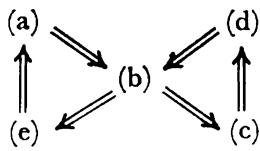
\includegraphics[keepaspectratio]{images/part003_cb91c25e.jpg}}

We show that (a) implies (b); if A is factorial, \(P^{*}\) is isomorphic to the group of divisors of A and hence to a direct sum of groups Z ( \(\S\) 1, no. 3, Theorem 2).

Note now that the relation ``the intersection of two integral principal ideals of A is a principal ideal'' means that every ordered pair of elements of A admits a lcm, that is that \(P^{*}\) is a lattice-ordered group (Algebra, Chapter VI, § 1, no. 9, Proposition 8). The fact that (b) implies (c) (and even is equivalent to it) therefore follows from Algebra, Chapter VI, § 1, no. 13, Theorem 2. The fact that (c) implies (d) follows from Algebra, Chapter VI, § 1, no. 13, Proposition 14 (DIV).

The fact that (d) implies (b) follows from Algebra, Chapter VI, § 1, no. 13, Theorem 2 applied to the group \(\mathcal{P}^*\) .

We show that (b) implies (e). If (b) holds, there is an isomorphism of \(\mathcal{P}^*\) onto \(\mathbf{Z}^{(I)}\) ; let \((v_{\iota}(x))_{\iota\in I}\) denote the element of \(\mathbf{Z}^{(I)}\) corresponding to the ideal \(Ax\) ( \(x\in K^*\) ). It is seen immediately that each \(v_{\iota}\) is a discrete valuation on \(\mathbf{K}\) , that \(\mathbf{A}\) is the intersection of the rings of the \(v_{\iota}\) and that, for \(x\in K^*\) , \(v_{\iota}(x)=0\) except for a finite number of indices \(\iota\) ; hence \(\mathbf{A}\) is a Krull domain. On the other hand, let \(q\) be a prime ideal of \(\mathbf{A}\) of height 1; it contains a non-zero element \(a\) which is necessarily not invertible and hence also (by definition of a prime ideal) one of the extremal elements \(p\) of \(\mathbf{A}\) ; as \(Ap\) is prime and non zero, \(q=Ap\) , which proves that \(q\) is principal.

Finally we show that (e) implies (a). Let \(\mathfrak{a}\) be a divisorial ideal of \(\mathbf{A}\) . There exist prime ideals \(p_i\) of \(\mathbf{A}\) of height 1 such that \(\operatorname{div} \mathfrak{a} = \sum_{i} n_i \operatorname{div} p_i\) where \(n_i \in \mathbf{Z}\) . If (e) holds, \(p_i\) is of the form \(A p_i\) , whence \(\operatorname{div} \mathfrak{a} = \operatorname{div}\left(\prod_{i} A p_i^{n_i}\right)\) and hence \(\mathfrak{a} = \prod_{i} A p_i^{n_i}\) since \(\mathfrak{a}\) is divisorial.

PROPOSITION 1. Let A be a Krull domain. If every divisorial ideal of A is invertible, then, for every maximal ideal m of A, \(A_{m}\) is factorial. The converse is true if it is also assumed that every divisorial ideal of A is finitely generated (in particular if A is Noetherian).

Suppose that every divisorial ideal of A is invertible; as \(A_{m}\) is a Krull domain (§ 1, no. 4, Proposition 6), every divisorial ideal a of \(A_{m}\) is the intersection of two principal fractional ideals (§ 1, no. 5, Corollary 2 to Proposition 9); hence \(a = bA_{m}\) , where b is a divisorial ideal of A (Chapter II, § 2, no. 4); as b is invertible by hypothesis, we deduce from Chapter II, § 5, no. 6, Theorem 4 that a is principal and hence \(A_{m}\) is a factorial domain (no. 1, Definition 1). Conversely, if all the \(A_{m}\) are factorial and c is a finitely generated divisorial ideal of A, \(cA_{m}\) is a divisorial ideal of \(A_{m}\) , as follows from § 1, no. 5, Corollary 2 to Proposition 9 and Chapter II, § 2, no. 4; by hypothesis \(cA_{m}\) is principal and hence it follows from Chapter II, § 5, no. 6, Theorem 4 that c is invertible.

